En esta sección se va a explicar cómo se ha entrenado el modelo de detección de estado del pavimento. Comenzaremos explicando los parámetros de entrenamiento y otras consideraciones que se deben tener en cuenta a la hora de entrenar un modelo de detección de objetos. Después, se explicará cómo se han preparado los datos de la CRDDC2022 para tener en cuenta estas consideraciones y adaptar los datos a las particularidades de la librería Ultralytics. Por último, se explicará los requerimientos de hardware necesarios para entrenar los modelos de detección de objetos y cómo se ha llevado a cabo el entrenamiento en Google Colab y en VPULab durante el desarrollo de este TFG.

\subsection{Parámetros de entrenamiento y otras consideraciones}
Al entrenar modelos de aprendizaje profundo, se busca lograr una buena generalización, altas puntuaciones de precisión y recall, así como un entrenamiento rápido y eficiente. En esta subsección, exploraremos los parámetros de entrenamiento y otras consideraciones clave para alcanzar estos objetivos en la detección de objetos.

En el caso de los modelos YOLO, se debe tener en cuenta el tamaño del modelo en número de parámetros, el tamaño de batch, el número de épocas de entrenamiento, la proporción de los datos anotados que se usa para entrenamiento y validación.

YOLOv8 de Ultralytics tiene varios tamaños de modelo que se pueden usar. Los tamaños disponibles son 'nano', 'small', 'medium', 'large' y 'very large'. Por lo general, para cualquier conjunto de datos, a mayor tamaño de modelo, mejor será la precisión del modelo y más latencia o tiempo de inferencia se necesitará. Además, a mayor tamaño de modelo, más memoria y tiempo de entrenamiento se necesitará. Por lo tanto, se debe elegir el tamaño de modelo que mejor se ajuste a las necesidades del proyecto. En la figura \ref{fig:yolo-comparison-plots}, extraída de la documentación de Ultralytics \cite{yolov8_ultralytics}, se puede ver una comparación de los tamaños de los modelos YOLO de Ultralytics. Las gráficas muestran que YOLOv8 es la versión de YOLO con mejor mAP50-95 y que a mayor tamaño de modelo, mejor es la precisión del modelo. En la gráfica de la derecha se muestra que el tamaño de modelo también afecta negativamente a la velocidad de inferencia. El modelo 'nano' es el más rápido, pero también el menos preciso, mientras que el modelo 'very large' es el más preciso, pero también el más lento y el 'large' es el mejor equilibrio entre precisión y velocidad.

% Mostramos la graphs/yolo-comparison-plots.png
\begin{figure}[H]
    \centering
    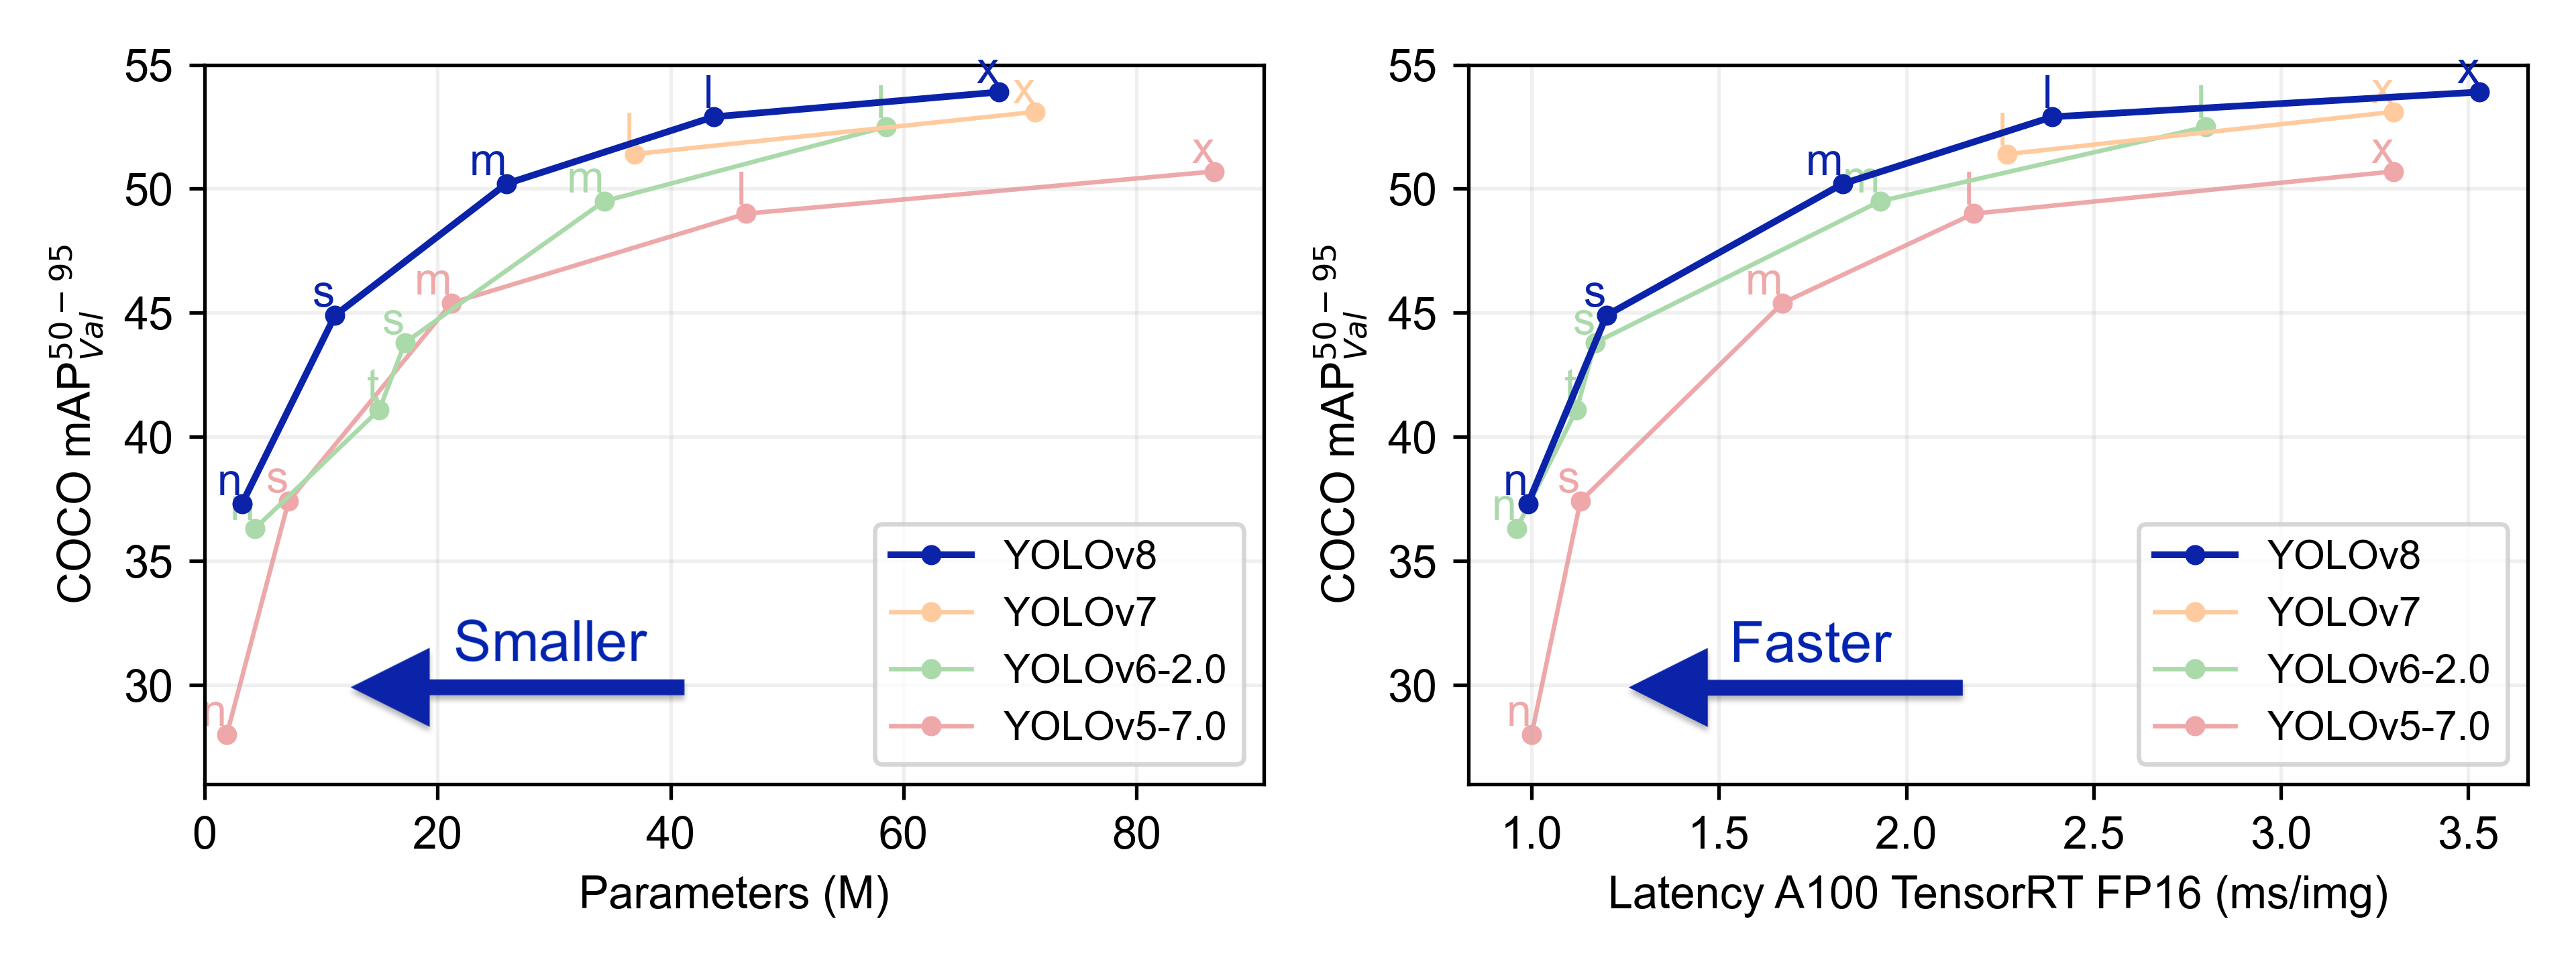
\includegraphics[width=0.9\textwidth]{graphs/yolo-comparison-plots.png}
    \caption{Comparación de los tamaños de los modelos YOLOv8 de Ultralytics.}
    \label{fig:yolo-comparison-plots}
\end{figure}

El número de épocas de entrenamiento y el tamaño de batch son dos hiperparámetros que determinan la cantidad de tiempo que se necesita para entrenar un modelo, la cantidad de memoria que se necesita y la velocidad de convergencia del modelo. Por lo general, a mayor número de épocas de entrenamiento, mejor será la precisión del modelo, pero también se corre el riesgo de sobreajustar el modelo al conjunto de entrenamiento. Por otro lado, a mayor tamaño de batch, más memoria se necesita, pero también se puede acelerar el entrenamiento. Por lo tanto, se debe elegir un número de épocas y un tamaño de batch que se ajuste a la capacidad de computación disponible. En el caso de los modelos de Computer Vision, la capacidad de computación suele ser la limitación más importante, ya que los modelos de detección de objetos suelen ser muy grandes y necesitan mucha memoria y tiempo para entrenar.

\subsection{Preparación de los datos}
En la sección de modelos [Sección \ref{SEC:MODELOS}] se ha explicado cómo se ha usado YOLO de Ultralytics para la detección del estado del pavimento. La elección de dicha librería nos obliga a realizar una serie de transformaciones en los datos para poder entrenar nuestros modelos. En esta subsección se va a explicar cómo se han preparado los datos de la CRDDC2022 para poder ser usados con YOLO de Ultralytics. Estos cambios se pueden encontrar detallados en los notebooks 'prepare-DatasetNinja.ipynb' y 'dataToYoloFormat.ipynb' en el repositorio del TFG \cite{TFG_Repository}.

Ultralytics requiere que las anotaciones tengan un formato especifico para poder ser usadas en el entrenamiento de los modelos. En concreto, las anotaciones deben estar en un directorio llamado 'labels' que esté en el mismo directorio que el directorio 'images' que contiene las imágenes. Cada archivo de anotación debe tener el mismo nombre que el archivo de imagen correspondiente, pero con extensión '.txt' en lugar de '.jpg'. El contenido de cada archivo de anotación debe tener una línea por cada objeto en la imagen con el siguiente formato:
\begin{center}
    \texttt{<clase> <x> <y> <width> <height>}
\end{center}
Donde \texttt{<clase>} es el índice de la clase del objeto, \texttt{<x>} y \texttt{<y>} son las coordenadas del centro de la caja delimitadora normalizadas, y \texttt{<width>} y \texttt{<height>} son el ancho y el alto de la caja delimitadora normalizados. Las coordenadas normalizadas se calculan dividiendo las coordenadas de la caja delimitadora por el ancho y el alto de la imagen, respectivamente. Esta transformación se han realizado con el notebook 'prepare-DatasetNinja.ipynb' en el repositorio del TFG \cite{TFG_Repository}. Se han realizado otros cambios menos significativos como reducir el tamaño de las imágenes de Noruega para que sea mas manejable en Google Colab.

\subsection{Entrenamiento en Google Colabs}
resumen .......

\subsection{Entrenamiento en VPULab}
resumen .......